\documentclass{standalone}
\usepackage{tikz}
\usetikzlibrary{patterns, positioning}


\begin{document}
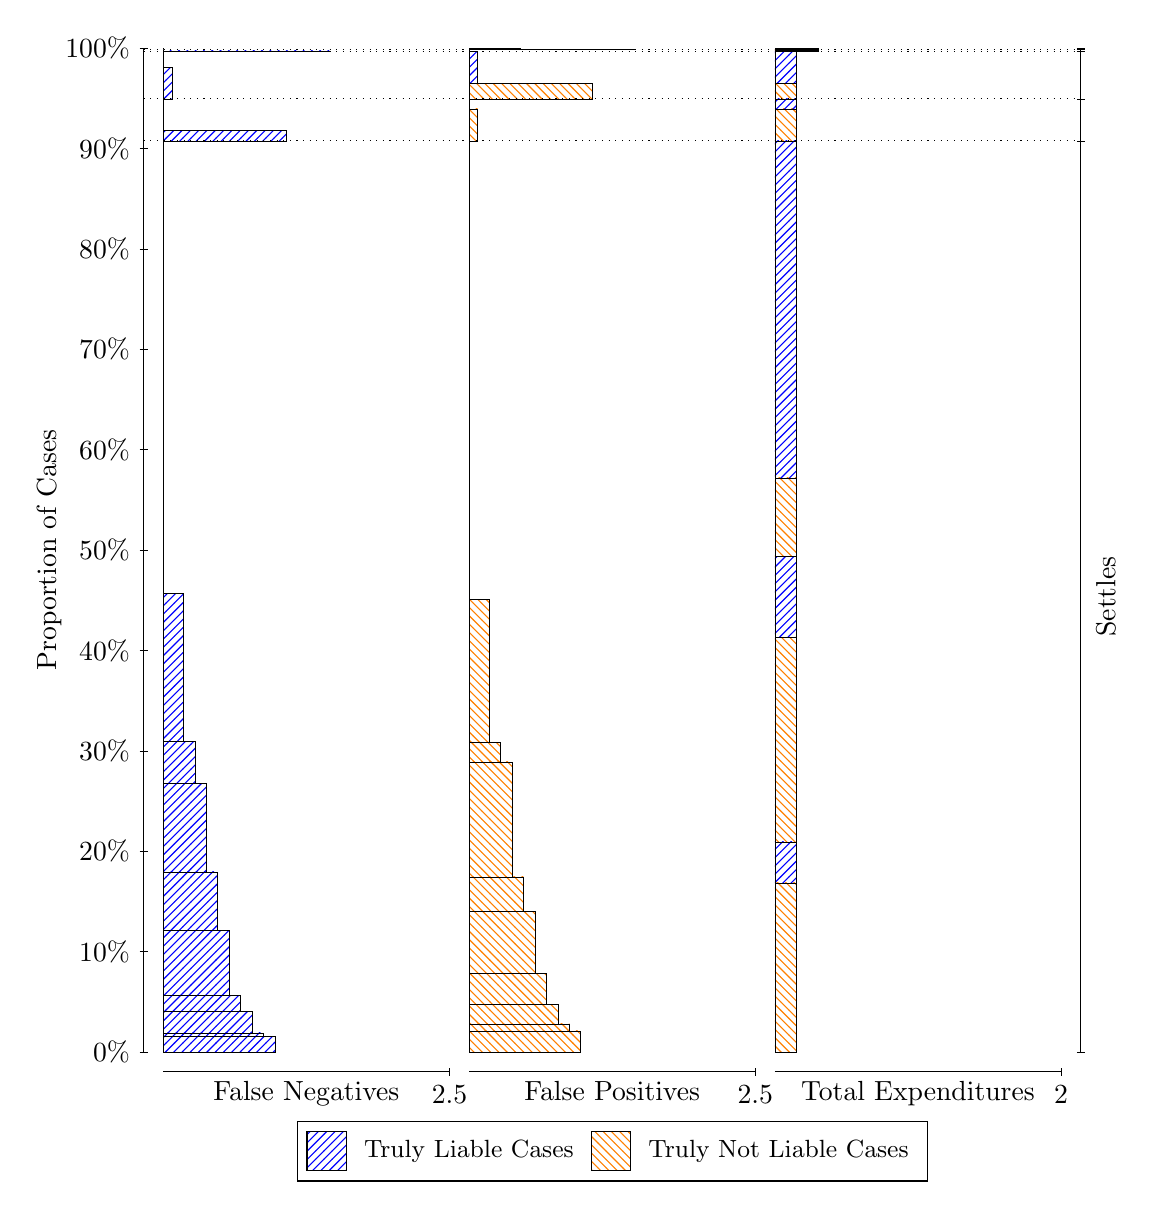
\begin{tikzpicture}
\draw[black, very thin] (1.5,1.75) -- (1.5,14.5);
\node[rotate=90, text=black, anchor=center] at (0.3, 8.125) {Proportion of Cases};
\draw[black, very thin] (1.45,1.75) -- (1.55,1.75);
\node[text=black, anchor=east] at (1.45, 1.75) {0\%};
\draw[black, very thin] (1.45,3.025) -- (1.55,3.025);
\node[text=black, anchor=east] at (1.45, 3.025) {10\%};
\draw[black, very thin] (1.45,4.3) -- (1.55,4.3);
\node[text=black, anchor=east] at (1.45, 4.3) {20\%};
\draw[black, very thin] (1.45,5.575) -- (1.55,5.575);
\node[text=black, anchor=east] at (1.45, 5.575) {30\%};
\draw[black, very thin] (1.45,6.85) -- (1.55,6.85);
\node[text=black, anchor=east] at (1.45, 6.85) {40\%};
\draw[black, very thin] (1.45,8.125) -- (1.55,8.125);
\node[text=black, anchor=east] at (1.45, 8.125) {50\%};
\draw[black, very thin] (1.45,9.4) -- (1.55,9.4);
\node[text=black, anchor=east] at (1.45, 9.4) {60\%};
\draw[black, very thin] (1.45,10.675) -- (1.55,10.675);
\node[text=black, anchor=east] at (1.45, 10.675) {70\%};
\draw[black, very thin] (1.45,11.95) -- (1.55,11.95);
\node[text=black, anchor=east] at (1.45, 11.95) {80\%};
\draw[black, very thin] (1.45,13.225) -- (1.55,13.225);
\node[text=black, anchor=east] at (1.45, 13.225) {90\%};
\draw[black, very thin] (1.45,14.5) -- (1.55,14.5);
\node[text=black, anchor=east] at (1.45, 14.5) {100\%};

\draw[black, very thin] (13.4,1.75) -- (13.4,14.5);
\draw[black, very thin] (13.35,1.75) -- (13.45,1.75);
\node[anchor=west] at (13.35, 1.75) {};
\draw[black, very thin] (13.35,13.322) -- (13.45,13.322);
\node[anchor=west] at (13.35, 13.322) {};
\draw[black, very thin] (13.35,13.855) -- (13.45,13.855);
\node[anchor=west] at (13.35, 13.855) {};
\draw[black, very thin] (13.35,14.456) -- (13.45,14.456);
\node[anchor=west] at (13.35, 14.456) {};
\draw[black, very thin] (13.35,14.48) -- (13.45,14.48);
\node[anchor=west] at (13.35, 14.48) {};
\draw[black, very thin] (13.35,14.5) -- (13.45,14.5);
\node[anchor=west] at (13.35, 14.5) {};

\draw[black, very thin, pattern color=blue, pattern=north east lines] (1.75,1.75) rectangle (3.167,1.9516);
\draw[black, very thin, pattern color=blue, pattern=north east lines] (1.75,1.9516) rectangle (3.0217,1.9914);
\draw[black, very thin, pattern color=blue, pattern=north east lines] (1.75,1.9914) rectangle (2.8763,2.2638);
\draw[black, very thin, pattern color=blue, pattern=north east lines] (1.75,2.2638) rectangle (2.731,2.4725);
\draw[black, very thin, pattern color=blue, pattern=north east lines] (1.75,2.4725) rectangle (2.5857,3.2956);
\draw[black, very thin, pattern color=blue, pattern=north east lines] (1.75,3.2956) rectangle (2.4403,4.0375);
\draw[black, very thin, pattern color=blue, pattern=north east lines] (1.75,4.0375) rectangle (2.295,5.1626);
\draw[black, very thin, pattern color=blue, pattern=north east lines] (1.75,5.1626) rectangle (2.1497,5.6902);
\draw[black, very thin, pattern color=blue, pattern=north east lines] (1.75,5.6902) rectangle (2.0043,7.5765);
\draw[black, very thin, pattern color=orange, pattern=north west lines] (1.75,7.5765) rectangle (1.75,13.322);
\draw[black, very thin, pattern color=blue, pattern=north east lines] (1.75,13.322) rectangle (3.3123,13.45);
\draw[black, very thin, pattern color=orange, pattern=north west lines] (1.75,13.45) rectangle (1.75,13.855);
\draw[black, very thin, pattern color=blue, pattern=north east lines] (1.75,13.855) rectangle (1.859,14.255);
\draw[black, very thin, pattern color=orange, pattern=north west lines] (1.75,14.255) rectangle (1.75,14.456);
\draw[black, very thin, pattern color=blue, pattern=north east lines] (1.75,14.456) rectangle (3.8573,14.463);
\draw[black, very thin, pattern color=orange, pattern=north west lines] (1.75,14.463) rectangle (1.75,14.48);
\draw[black, very thin, pattern color=orange, pattern=north west lines] (1.75,14.48) rectangle (1.75,14.487);
\draw[black, very thin, pattern color=blue, pattern=north east lines] (1.75,14.487) rectangle (1.75,14.5);
\draw[black, very thin, pattern color=orange, pattern=north west lines] (5.6333,1.75) rectangle (7.0503,2.019);
\draw[black, very thin, pattern color=orange, pattern=north west lines] (5.6333,2.019) rectangle (6.905,2.1072);
\draw[black, very thin, pattern color=orange, pattern=north west lines] (5.6333,2.1072) rectangle (6.7597,2.3532);
\draw[black, very thin, pattern color=orange, pattern=north west lines] (5.6333,2.3532) rectangle (6.6143,2.7485);
\draw[black, very thin, pattern color=orange, pattern=north west lines] (5.6333,2.7485) rectangle (6.469,3.5377);
\draw[black, very thin, pattern color=orange, pattern=north west lines] (5.6333,3.5377) rectangle (6.3237,3.9746);
\draw[black, very thin, pattern color=orange, pattern=north west lines] (5.6333,3.9746) rectangle (6.1783,5.4327);
\draw[black, very thin, pattern color=orange, pattern=north west lines] (5.6333,5.4327) rectangle (6.033,5.6843);
\draw[black, very thin, pattern color=orange, pattern=north west lines] (5.6333,5.6843) rectangle (5.8877,7.4953);
\draw[black, very thin, pattern color=blue, pattern=north east lines] (5.6333,7.4953) rectangle (5.6333,13.322);
\draw[black, very thin, pattern color=orange, pattern=north west lines] (5.6333,13.322) rectangle (5.7423,13.727);
\draw[black, very thin, pattern color=blue, pattern=north east lines] (5.6333,13.727) rectangle (5.6333,13.855);
\draw[black, very thin, pattern color=orange, pattern=north west lines] (5.6333,13.855) rectangle (7.1957,14.055);
\draw[black, very thin, pattern color=blue, pattern=north east lines] (5.6333,14.055) rectangle (5.7423,14.456);
\draw[black, very thin, pattern color=orange, pattern=north west lines] (5.6333,14.456) rectangle (5.6333,14.473);
\draw[black, very thin, pattern color=blue, pattern=north east lines] (5.6333,14.473) rectangle (5.6333,14.48);
\draw[black, very thin, pattern color=orange, pattern=north west lines] (5.6333,14.48) rectangle (7.7407,14.487);
\draw[black, very thin, pattern color=blue, pattern=north east lines] (5.6333,14.487) rectangle (6.2873,14.5);
\draw[black, very thin, pattern color=orange, pattern=north west lines] (9.5167,1.75) rectangle (9.7892,3.8966);
\draw[black, very thin, pattern color=blue, pattern=north east lines] (9.5167,3.8966) rectangle (9.7892,4.4175);
\draw[black, very thin, pattern color=orange, pattern=north west lines] (9.5167,4.4175) rectangle (9.7892,7.0177);
\draw[black, very thin, pattern color=blue, pattern=north east lines] (9.5167,7.0177) rectangle (9.7892,8.0424);
\draw[black, very thin, pattern color=orange, pattern=north west lines] (9.5167,8.0424) rectangle (9.7892,9.0409);
\draw[black, very thin, pattern color=blue, pattern=north east lines] (9.5167,9.0409) rectangle (9.7892,13.322);
\draw[black, very thin, pattern color=orange, pattern=north west lines] (9.5167,13.322) rectangle (9.7892,13.727);
\draw[black, very thin, pattern color=blue, pattern=north east lines] (9.5167,13.727) rectangle (9.7892,13.855);
\draw[black, very thin, pattern color=orange, pattern=north west lines] (9.5167,13.855) rectangle (9.7892,14.055);
\draw[black, very thin, pattern color=blue, pattern=north east lines] (9.5167,14.055) rectangle (9.7892,14.456);
\draw[black, very thin, pattern color=orange, pattern=north west lines] (9.5167,14.456) rectangle (10.062,14.473);
\draw[black, very thin, pattern color=blue, pattern=north east lines] (9.5167,14.473) rectangle (10.062,14.48);
\draw[black, very thin, pattern color=orange, pattern=north west lines] (9.5167,14.48) rectangle (10.062,14.487);
\draw[black, very thin, pattern color=blue, pattern=north east lines] (9.5167,14.487) rectangle (10.062,14.5);
\draw[black, dotted] (1.5,13.322) -- (13.4,13.322);
\draw[black, dotted] (1.5,13.855) -- (13.4,13.855);
\draw[black, dotted] (1.5,14.456) -- (13.4,14.456);
\draw[black, dotted] (1.5,14.48) -- (13.4,14.48);
\draw[black, very thin] (1.75,1.5) -- (5.3833,1.5);
\node[text=black, anchor=north] at (3.5667, 1.5) {False Negatives};
\draw[black, very thin] (5.3833,1.45) -- (5.3833,1.55);
\node[text=black, anchor=north] at (5.3833, 1.45) {2.5};

\draw[black, very thin] (5.6333,1.5) -- (9.2667,1.5);
\node[text=black, anchor=north] at (7.45, 1.5) {False Positives};
\draw[black, very thin] (9.2667,1.45) -- (9.2667,1.55);
\node[text=black, anchor=north] at (9.2667, 1.45) {2.5};

\draw[black, very thin] (9.5167,1.5) -- (13.15,1.5);
\node[text=black, anchor=north] at (11.333, 1.5) {Total Expenditures};
\draw[black, very thin] (13.15,1.45) -- (13.15,1.55);
\node[text=black, anchor=north] at (13.15, 1.45) {2};

\node[text=black, centered, rotate=90] at (13.72, 7.5359) {Settles};





\draw (7.449999999999999,1.5) node[draw=none] (baseCoordinate) {};
\begin{scope}[align=center]
        \matrix[scale=0.5, draw=black, below=0.5cm of baseCoordinate, nodes={draw}, column sep=0.1cm]{
            \node[rectangle, draw, minimum width=0.5cm, minimum height=0.5cm, pattern color=blue, pattern=north east lines] {}; &
            \node[draw=none, font=\small, text=black] (B) {Truly Liable Cases}; &
            \node[rectangle, draw, minimum width=0.5cm, minimum height=0.5cm, pattern color=orange, pattern=north west lines] {}; &
            \node[draw=none, font=\small, text=black] (B) {Truly Not Liable Cases}; \\
            };
\end{scope}

\end{tikzpicture}
\end{document}